\chapter{評価実験}
提案手法の有効性を示すため2種類の実験を行った.いずれもタスクの対象としてconnect4を扱っている.\\
一つ目の実験(以下データ実験と表記)はコンピュータ同士の対戦データを用いて提案手法による想定図の妥当性の実証を試みた.\\
二つ目の実験(以下システム実験と表記)は自作のconnect4学習支援システムを用いて提案手法のユーザーインタフェースを含んだ優位性の実証を試みた.
この章ではまず実験の際に用いたタスクであるconnect4と使用したモデルであるalphazero\_baselineについて述べる.そののちにデータ実験,システム実験の詳細と結果を記載する.
\section{connect4}
connect4\cite{connect4}はボードゲームの一種である.ルールは五目並べに極めて近く,図\ref{fig:connect4}の右側の画像のように、二人のプレイヤーが交互に互いの駒を盤上に置き,最終的に縦・横・もしくは斜めに連続して4つの石を並べたプレイヤーの勝利となる.ただし,五目並べや連珠との相違点として「重力」の存在が挙げられる.
この「重力」とは各プレイヤーが石をボード上の最も下の行または既に置かれた石の上にしか置けないという規則を表している.そのため,各プレイヤーの選択肢はボードの列の数と等しい.
図\ref{fig:connect4}の左側は左から5番目の列を指定した際に、石がボード上の最下の列に置かれる様子を示している。
connect4の一般的なボードの広さは$6\times7$であり$6\times7$のコネクト4については1988年にAllis\cite{allis}により知識ベースの手法による先番勝利が証明された.
Tromp\cite{data}によるconnect4の$\alpha-\beta$木探索によって導かれた各盤面の最善手とそのデータも一般に公開されている.
また,connect4は盤上に全ての情報が開示されており,結果もどちらか一方の勝利または引き分けのみであるため2人ゼロ和完全情報ゲームに分類される.
本論文の実験において提案手法をconnect4に適用する際には最終盤面において4つ以上並んでいる石の座標を特徴として用いた.
\begin{figure}[t]
	\centering
    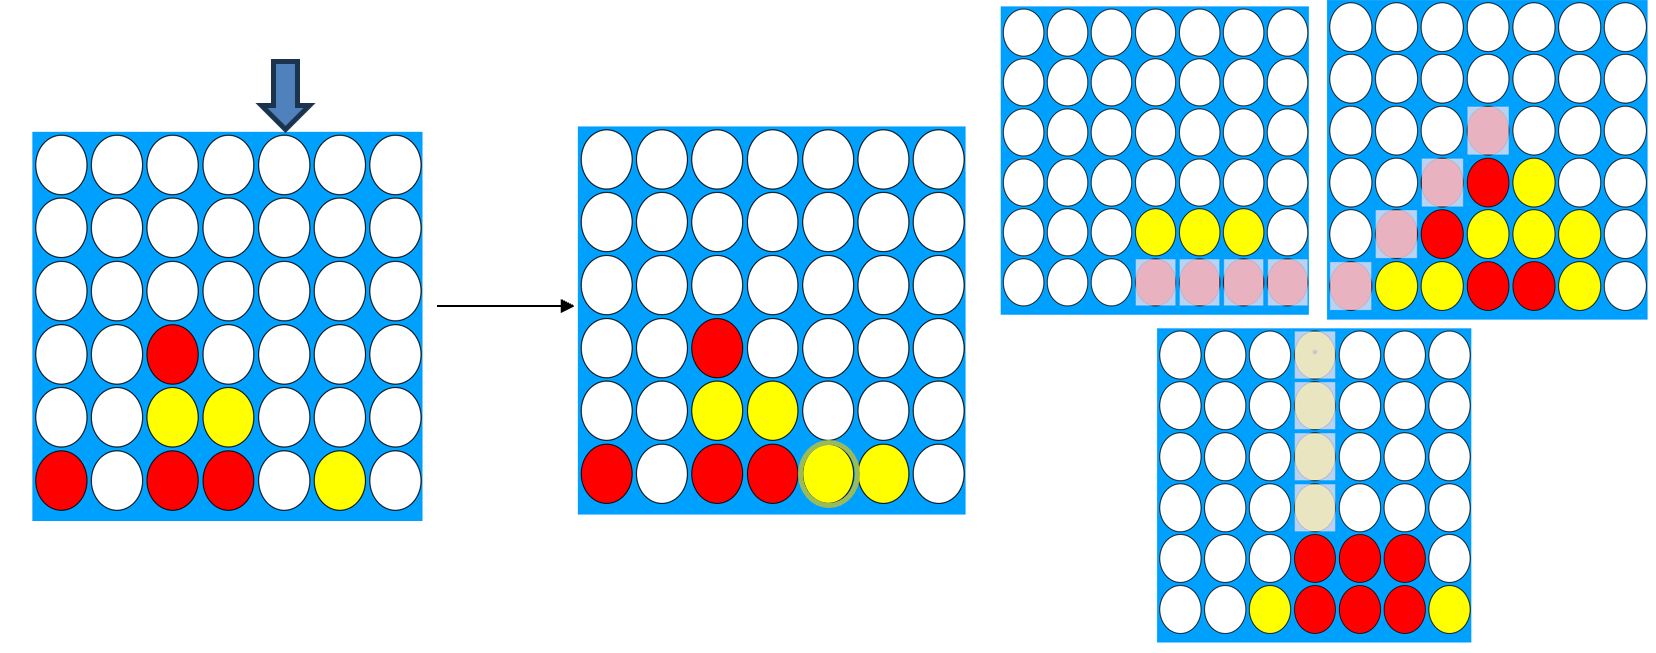
\includegraphics[width=\linewidth]{./figure/connect4.png}
	\caption{connect4}
	\label{fig:connect4}
\end{figure}
\section{alphazero\_baseline}
alphazero\_baseline\cite{baseline}はalphaZeroをconnect4用に簡易的に模したネットワークであり,図\ref{fig:baseline}に示すように入力は最新の盤面$s_0$,出力は$1\times7$(7はボードの列の数)の方策$P(s)(以下s=s_0とする)$とスカラー値の局面評価$V(s)$(値域は-1から1)である.
方策は確率分布であり,要素の値が大きいインデックスを選択することで勝利に近づくと予想される.
局面評価は第2章の強化学習の段で記載した状態価値関数と同一の変数であり,
入力に対する評価を表しており,1が入力の手番のプレイヤーにとっての勝利,-1が敗北の予想を表している.

\begin{figure}[t]
    \centering
    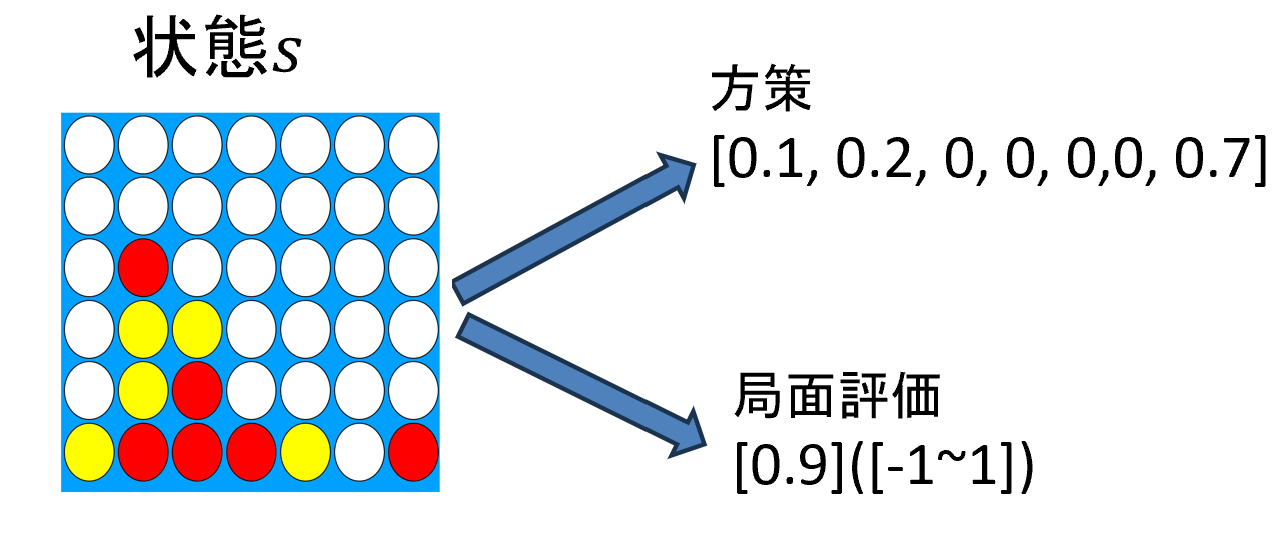
\includegraphics[trim={0cm 0cm 0cm 0cm},clip]{./figure/baseline.png}

    \caption{alphazero\_baselineの入出力}
    \label{fig:baseline}
\end{figure}


\section{データ実験}
\label{chap:evaluation}
提案手法と後に述べる比較手法によるゲーム結果(後で勝敗も含める)の予測精度を比較した.
\subsection{データセット}
alphazero\_baselinモデル同士の対戦データ2000局分(盤面数:61049)を使用した.いずれもいずれも弱いAIが先番のデータを使用している.これは弱いAIが後番の場合評価関数の変動が極めて小さくなることと,弱い側が先番を選択することが指導において一般的とされるためである.

\subsection{比較手法}
提案手法と比較手法はそれぞれ以下の方式で予測を行う.
比較手法の詳細なアルゴリズムは付録\ref{chap:alg}に記載した.
\newpage
\begin{itemize}
	\item 比較手法: 探索の開始地点から最も訪問回数が大きい選択肢を選び,決定木の端までたどり着いた際にそこで四つ繋がっている石の組み合わせ,位置を記録する.
	\item 提案手法: 集めた盤面における4つ繋がっている石を集計し,出現頻度が高い4つの個別の石の位置と出現頻度が高い二つの組み合わせを記録する.組み合わせを二つ記録する理由は下の図のように最終的に繋がっている組み合わせが二つある可能性を考慮するためである.
\end{itemize}
図\ref{fig:compare}は比較手法と提案手法の概要を示している.
\begin{figure}[t]
	\centering
	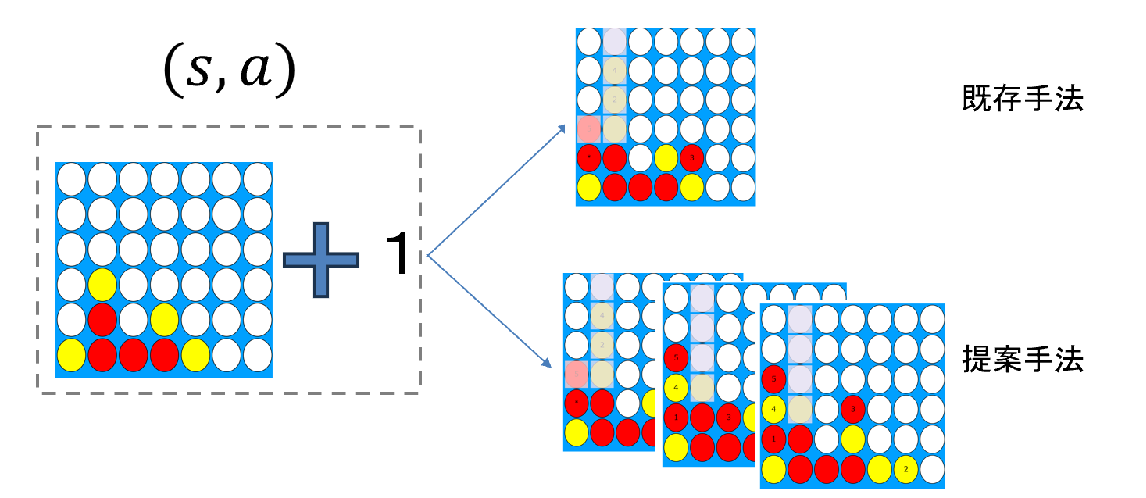
\includegraphics[width=\linewidth]{./figure/compare.pdf}
	\caption{提案手法と比較手法の比較}
	\label{fig:compare}
\end{figure}

\subsection{評価指標}
両手法による予測の精度を独自に定義した二つの定義group count($C_g$),stone count($C_s$)によって計測した.stone count, group countの詳細な定義は付録Aに記載する.
それぞれが,最終盤面において4つ以上連続して並ぶ石と組み合わせ(以下fatal stone,fatal groupと記載)の座標に対する予測精度を表している.
ここでは概略を述べる.
手法によって予測されたfatal stone,fatal groupの座標をそれぞれ$F_s, F_g$とする.

\paragraph{group count}~
\par 予測の石の組み合わせ単位での精度を示しており,
手法による予測$F_g$と実際のfatal groupの集合$R_g$に共通する要素がある場合1,無い場合は0となる.
また,$F_g$と$R_g$が両方とも空集合$\phi$である場合(実際の結果が引き分けでありかつそれを正しく予測できている場合)group countは1となる.
\paragraph{stone count}~
\par 予測の個別の石単位での精度を表しており,
手法による予測$F_s$と実際の集合$R_s$の共通する要素の数を4で割った値である.値の最大値は1であり,先述の値が1を超える場合もstone countは1として扱う.
group countと同様に$F_s$と$R_s$が両方とも空集合である場合stone countは1となる.
\subsection{実験結果}
盤面データのうち,手数(盤面上の赤または黄色)が13$\sim$24のものに対して実験を行った.
表\ref{table:result-online}に実験結果を示す.いずれの場合もgroup countにおいて提案手法は比較手法より高い値を示した.
表中に記載した「補間」の詳細は付録\ref{chap:alg}に記載する.
\begin{table}[H]
	\caption{実験結果:データ実験}
	\centering
	\scalebox{0.98}[0.98]{
		\begin{tabular}{c|c|c|c|c}
			\multicolumn{1}{c}{} & \multicolumn{2}{|c|}{group count} 
			& \multicolumn{2}{c|}{stone count}\\ \hline \hline
			手数(盤面数, 補間の有無)    & 提案手法 & 比較手法 & 提案手法 & 比較手法 \\ \hline
			19-24(9862, 無)    & \bf{0.60} & 0.43 & 0.55 & \bf{0.62} \\
			19-24(9862, 有)    & \bf{0.63} & 0.44 & 0.61 & \bf{0.63}  \\
			13-24(21022, 無)   & \bf{0.52} & 0.37 & 0.55 & \bf{0.56}  \\
			13-24(21022, 有)   & \bf{0.55} & 0.37 & 0.55 & \bf{0.56}  \\
		\end{tabular}
	}
	\label{table:result-online}
\end{table}
\subsection{考察(データ実験)}
提案手法はgroup countにおいて比較手法より高い結果を示した.
この結果は提案手法がfatal groupを予測する能力に長けている事を意味する.
比較手法によって予測されるfatal groupの集合は
最も訪問回数が大きい分岐が辿り着く1つの最終状態のものである.
一方で提案手法により予測されるfatal groupの集合は,複数の分岐がそれぞれに辿り着く最終状態のfatal groupの多数派投票によって決定され,第1位と第2位のものが採用される.\\
使用した対戦データは対戦者間の強さに差があり,予測は強い側の決定木を用いている.
決定木内での最も訪問回数の大きい分岐(以下主分岐と記載)はAIが予測する双方が最善を尽くした場合の進行と解釈される.
実際に弱いAIと対戦を行う際には,弱いAIは強いAIが最善とみなす行動(最も訪問回数が大きい行動)を必ずしも選択しない.
そのため,実際の進行は,比較手法に用いられる主分岐とは異なる可能性が高い.
提案手法では,主分岐を含む複数の分岐を用いているため,より精度の高い予測が可能になったと考えられる.\\
また,提案手法は2組のfatal groupを保存することから比較手法よりも予測するfatal groupの数が多くなる傾向にあるため,必然的にgroup countの値も大きくなったとも考えられる.


\section{システム実験}
提案手法の人間に対する有効性を示すため以下のように自作したconnect4の学習支援システムを用いて実験を行った.
自作システムの開始画面は\ref{fig:basic}のように構成されており,右側の青い正方形の部分をクリックすることでconnect4をプレイできる.
実験対象者は計22人の10代-20代学生(男性17名:女性5名)となった.
\begin{figure}[t]
	\centering
	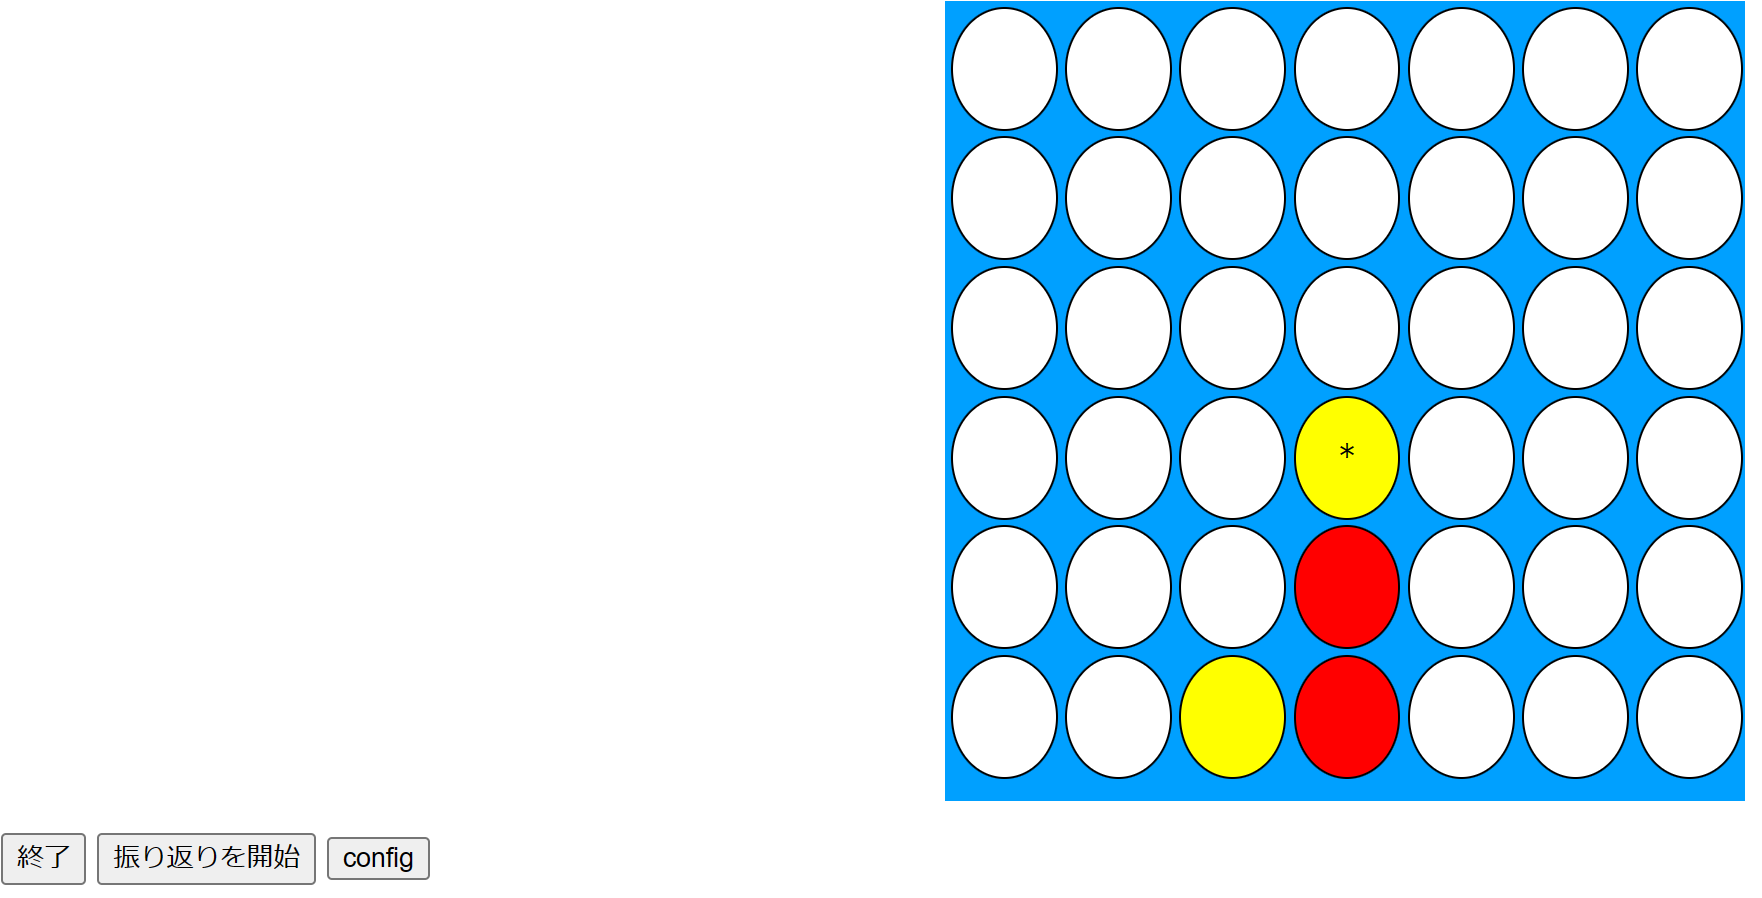
\includegraphics[width=\linewidth]{./figure/basicSystem.png}
	\caption{開始画面}
	\label{fig:basic}
\end{figure}
\subsection{実験手順}
実験は被験者一人あたりにつき三回行われ,前半二回を第一段階(提案手法による学習),後半一回が第二段階(被験者同士の対戦)とした.
ここでは第一段階である提案手法の学習について述べる.
\newpage
\paragraph{第一段階(提案手法による学習)}~
\par 提案システムを用いた学習はさらに
\begin{itemize}
	\item AIシステム(alphazero\_baseline)との対戦
	\item 提案手法によるゲームの振り返り
\end{itemize}
の2ステップに分けられる.AIシステムとの対戦が終了するとシステムは「振り返りモード」に移行する.
「振り返りモード」は図\ref{fig:lookBack}のように構成され,右側に直前のゲームの振り返りたい地点の盤面が表示され,ユーザーは各種ボタンを押すことで
AIによる進行図を閲覧できる.進行図は提案手法または比較手法によって生成される.
インタフェースの詳しい構成は付録\ref{chap:system}に記載した。
また、「振り返りモード」は第3章で定義した重要度$I(s)$が最も高い地点から開始する.

実験の際には被験者をグループA(提案手法による進行図を見せるグループ)とグループB(比較手法による進行図を見せるグループ)に分類した.
\begin{figure}[t]
	\centering
	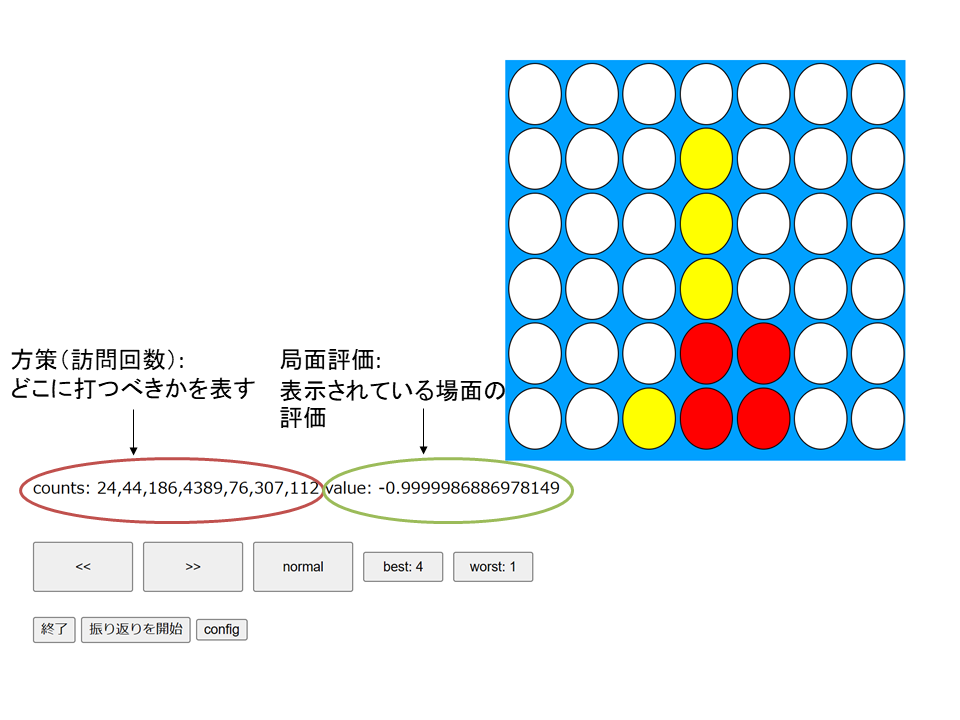
\includegraphics[width=\linewidth]{./figure/lookBack.png}
	\caption{振り返り画面}
	\label{fig:lookBack}
\end{figure}
数字が描かれたボタンは列のインデックスを表しており,図\ref{fig:trajSystem}に示すように各ボタンを押した際にその列を選択した場合の想定図と局面評価を確認できる.
\begin{figure}[t]
    \centering
    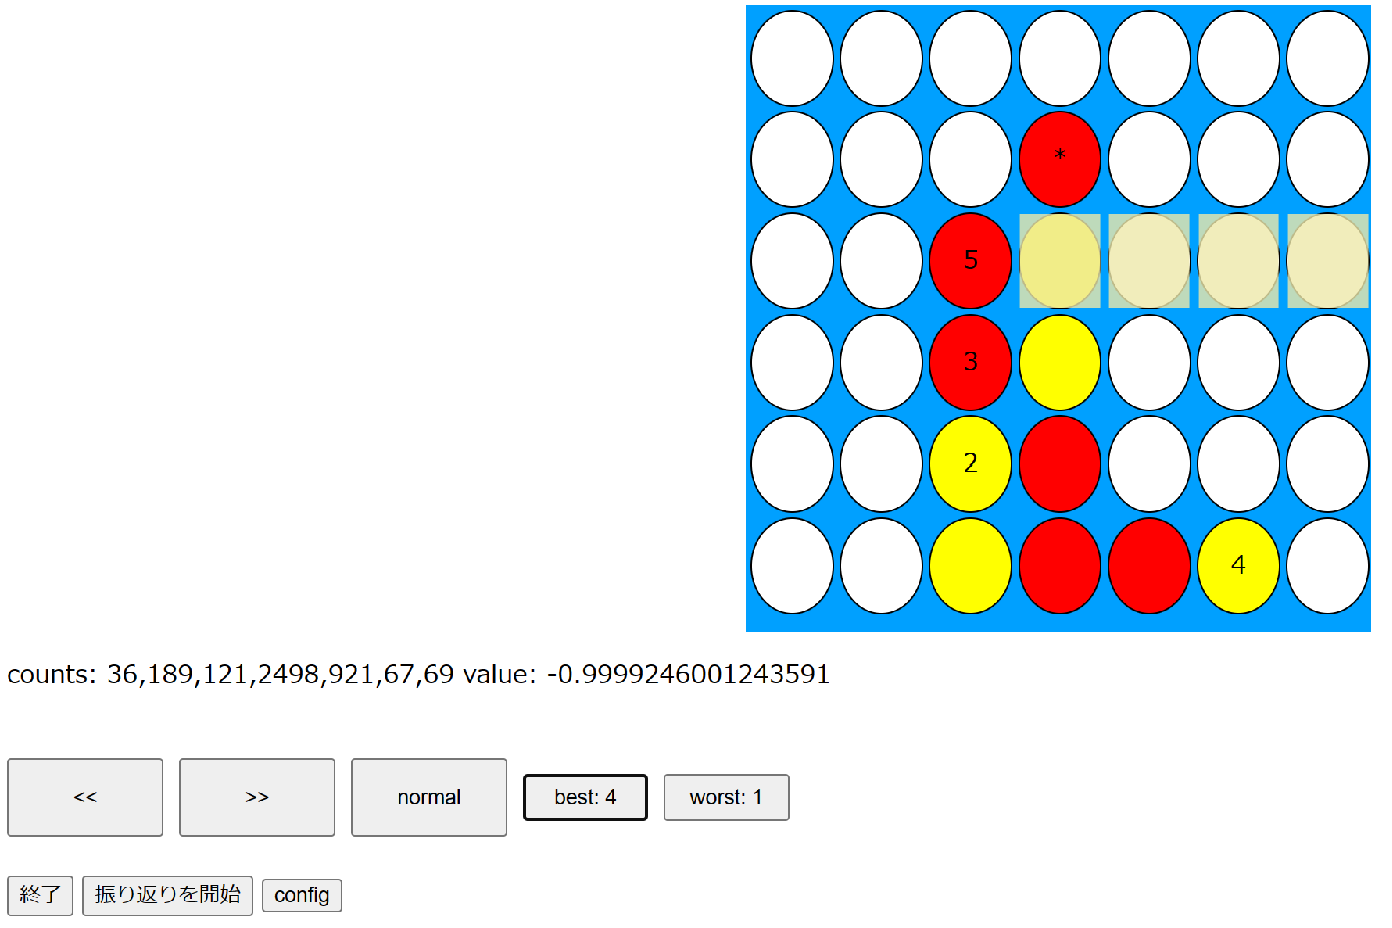
\includegraphics[width=\linewidth]{./figure/trajSystem.pdf}
	\caption{進行図の表示}
	\label{fig:trajSystem}
\end{figure}
\subsection{評価指標}
システム実験の評価指標は主観評価と客観評価の二つに分けられる.
主観評価は被験者による五段階評価であり,「タスクの熟達度に関連する質問」((a))と「タスクの楽しさ・面白さに関連する質問」((b))の二つに分けられる.
具体的な質問事項は付録Dに記載する.
客観評価はグループA(提案手法)の被験者とグループB(比較手法)の被験者の対戦成績である.

\subsection{実験結果}
進行図で提示される先読みの手数ごとに主観評価の平均値($1\sim5$)を表\ref{table:system-3}, 表\ref{table:system-5}, 表\ref{table:system-7}, 表\ref{table:system-100}に示す.
先読みの手数は${3, 5, 7, \textrm{制限なし}}$の四種類であり,先読みの手数ごとに図\ref{fig:see}に示すように提示される進行図中の手数が変化する.
先読みの手数に関わらず,AIが予測する進行において最終的に4つ以上の石が並ぶ座標は強調表示される.
\begin{figure}[t]
    \centering
    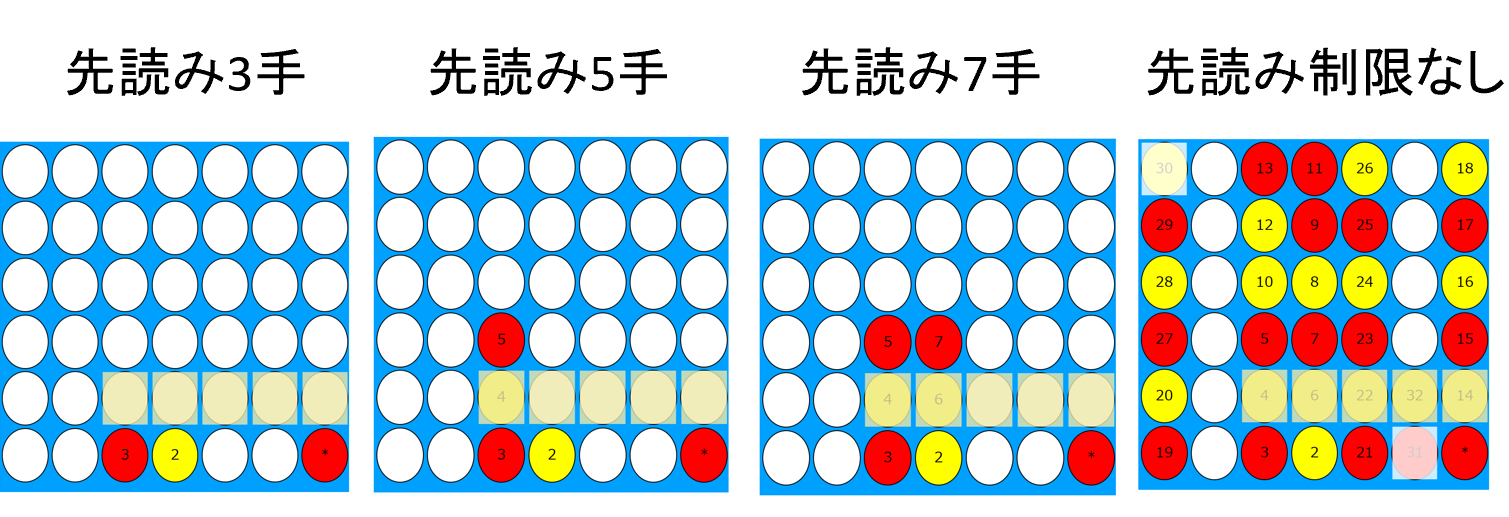
\includegraphics[width=\linewidth]{./figure/see.png}
	\caption{進行図の表示}
	\label{fig:see}
\end{figure}
先読み手数が3手または先読み手数制限なしの場合に,提案手法は比較手法に対して高い結果を示した.
\begin{table}[H]
    \caption{先読み手数3手の場合}
    \label{table:system-3}
    \scriptsize
    \centering
    \resizebox{\linewidth}{!}{
        \begin{tabular}{c|l||c|c}
            \multicolumn{2}{c}{質問} & \multicolumn{2}{c}{主観評価} \\ \hline \hline
            質問の種類 & 質問の内容 & A & B \\ \hline 
            (a) & 振り返りによって成長したと感じましたか & \bf{3.29} & 3.17 \\
            & 振り返りによってAIの意図を掴むことができたと感じますか & 2.43 & \bf{2.67} \\
            & (二回目のみ) 一回目に比べて成長したと感じますか & 2.75 & \bf{4.33} \\ \hline
            (b) & 今後も connect4 をプレイするときにこのシステムを使いたいと思いましたか & \bf{3.71} & 3.67 \\
            & システムにより振り返りが楽しくなったと感じますか & {3.57} & \bf{3.60} \\
        \end{tabular}
    }
    
\end{table}
\begin{table}[H]
    \caption{先読み手数5手の場合}
    \scriptsize
    \centering
    \resizebox{\linewidth}{!}{
        \begin{tabular}{c|l||c|c}
            \multicolumn{2}{c}{質問} & \multicolumn{2}{c}{主観評価} \\ \hline \hline
            質問の種類 & 質問の内容 & A & B \\ \hline 
            (a) & 振り返りによって成長したと感じましたか & 3.00 & \bf{4.00} \\
            & 振り返りによってAIの意図を掴むことができたと感じますか & 2.60 & \bf{4.00} \\
            & (二回目のみ) 一回目に比べて成長したと感じますか & 3.67 & \bf{4.33} \\ \hline
            (b) & 今後も connect4 をプレイするときにこのシステムを使いたいと思いましたか & 4.00 & \bf{4.80} \\
            & システムにより振り返りが楽しくなったと感じますか & 4.20 & \bf{4.60} \\
        \end{tabular}
    }
    \label{table:system-5}
\end{table}
\begin{table}[H]
    \caption{先読み手数7手の場合}
    \scriptsize
    \centering
    \resizebox{\linewidth}{!}{
        \begin{tabular}{c|l||c|c}
            \multicolumn{2}{c}{質問} & \multicolumn{2}{c}{主観評価} \\ \hline \hline
            質問の種類 & 質問の内容 & A & B \\ \hline 
            (a) & 振り返りによって成長したと感じましたか & {3.83} & \bf{4.33} \\
            & 振り返りによってAIの意図を掴むことができたと感じますか & 2.67 & \bf{3.67} \\
            & (二回目のみ) 一回目に比べて成長したと感じますか & 2.75 & \bf{4.33} \\ \hline
            (b) & 今後も connect4 をプレイするときにこのシステムを使いたいと思いましたか & 4.17 & \bf{4.67} \\
            & システムにより振り返りが楽しくなったと感じますか & 3.00 & \bf{3.50} \\
        \end{tabular}
    }
    \label{table:system-7}
\end{table}
\begin{table}[H]
    \caption{先読み手数制限なしの場合}
    \scriptsize
    \centering
    \resizebox{\linewidth}{!}{
        \begin{tabular}{c|l||c|c}
            \multicolumn{2}{c}{質問} & \multicolumn{2}{c}{主観評価} \\ \hline \hline
            質問の種類 & 質問の内容 & A & B \\ \hline 
            (a) & 振り返りによって成長したと感じましたか & \bf{4.25} & 4.00 \\
            & 振り返りによってAIの意図を掴むことができたと感じますか & \bf{3.50} & 3.00 \\
            & (二回目のみ) 一回目に比べて成長したと感じますか & 2.75 & \bf{4.33} \\ \hline
            (b) & 今後も connect4 をプレイするときにこのシステムを使いたいと思いましたか & \bf{4.5} & 4.00 \\
            & システムにより振り返りが楽しくなったと感じますか & \bf{4.75} & 4.40 \\
        \end{tabular}
    }
    \label{table:system-100}
\end{table}
また,第二段階である被験者同士の対戦結果を表\ref{table:result-battle}に示す.
付録Dに示すように被験者一人に対して二回対戦を行った.結果として示すscoreは勝利を1,敗北を-1,引き分けを0
とした二回の対戦の平均値として定義される.
提案手法を用いて訓練を行ったグループ(A)は比較手法を用いて訓練を行ったグループ(B)よりも高い
勝率を記録した.
\begin{table}[H]
	\caption{対戦の結果}
    \label{table:result-battle}
	\centering
	\scalebox{0.98}[0.98]{
		\begin{tabular}{c|c}
			グループ & score \\ \hline
			A(提案手法)    & \bf{0.25} \\ 
			B(比較手法)    & -0.15 \\
		\end{tabular}
	}
	
\end{table}
また,第三章で示した新たな重要度の定義(式\ref{new-imp})の妥当性を検証するため,盤面$s$の重要度$I(s)$と被験者が$s$の進行図を
見た時間$t$の相関を調査した.比較手法には式\ref{imp}の定義を用いた.
結果を表\ref{table:result-imp}に示す.いずれの手法も$t$との有意な相関が見られなかった.
\begin{table}[H]
	\caption{重要度と$t$の相関}
    \label{table:result-imp}
	\centering
	\scalebox{0.98}[0.98]{
		\begin{tabular}{c|c|c}
			日数& 提案手法 & 比較手法 \\ \hline
			1日目& {-0.035}& \bf{-0.034}\\
            2日目& {-0.083}& \bf{0.067}\\
		\end{tabular}
	}
	
\end{table}


\subsection{考察(システム実験)}


提案手法を用いたグループAがグループBを上回る評価を得たのは,主に先読みが最も短い3手の場合と最も長い制限なしの場合となった.

先読み3手・制限なしの場合のデータをさらに1日目,2日目で分類した結果,
\begin{itemize}
    \item 先読み3手の場合は1日目
    \item 先読み制限なしの場合は2日目
\end{itemize}

の方がよりグループAからの評価が高いことが分かった.
付録\ref{chap:system}で述べるように,1日目と2日目ではGUIの設定に差があり
1日目のGUIでは全ての選択肢(最大7種)を起点とした進行図を閲覧可能であるのに対し,2日目のGUIでは起点となる選択肢を
二つに制限した.
そのため,2日目は被験者が見られる進行図の数が1日目の約$\frac{1}{3}$となる.

そのため,「1日目・先読み3手の場合」と「2日目・先読み制限なし」の場合に被験者が受け取る情報量は近しいと推測される.

また,データを「被験者のグループ・日にち・先読み手数」によって分類し,「振り返りによってAIの意図を掴むことができたと感じますか」という質問に対する評価(以下把握満足度と表記)の降順に
並べ直した結果を表\ref{table:order}に示す.
\begin{table}[H]
	\caption{把握満足度}
    \label{table:order}
    \scriptsize
	\centering
	\scalebox{0.98}[0.98]{
		\begin{tabular}{c|c|c||c}
			グループ& 日 & 先読み手数 &把握満足度 \\ \hline
			B & 2 & 5 & 4.67\\
            B & 2 & 7 & 4.00\\
            A & 1 & 制限なし& 3.50\\
            A & 2 & 制限なし& 3.50\\
            B & 1 & 3& 3.50\\
            B & 1 & 制限なし& 3.33\\
            A & 1 & 3& 3.33\\
            \multicolumn{4}{c}{(\ldots)}\\
            A & 2 & 3 & 1.75\\
            B & 1 & 3 & 1.50\\

		\end{tabular}
	}
	
\end{table}

グループAのデータを日にちと先読み手数で分けた場合最も把握満足度が高いのは
「2日目・先読み制限なし」,次いで「1日目・先読み制限なし」,「1日目・先読み3手」となった.
最も情報が少ない「2日目・3手」はグループAの全8パターン中最下位となった.\\


グループBに対しても同様に「振り返りによってAIの意図を掴むことができたと感じますか」への評価を集計した結果,
最も評価が高いのは「2日目・5手」,次いで「2日目・7手」,「1日目・3手」となった.\\



また,付録\ref{chap:data}の表\ref{table:tail}より提案手法が示す1組の状態$s$,行動$a$について示す分岐の数$n$の平均は約10であるため,比較手法が示す情報量は提案手法の約$\frac{1}{10}$となる.
また,先読みの手数に制限が無い場合の手数の平均は約15手である.
そのため提示する情報量が大きい程評価が高くなるわけではなく,手法ごとに被験者が適切と感じる情報量が存在すると推測される.\\

以上の考察
を踏まえて,被験者に対して提示する情報を最小化した上で適切な情報量を調査するため,
先読みを1$\sim$5手として再実験を行った.
システム実験では補助として提示した訪問回数,局面評価に注目する被験者が多く見られたため,訪問回数「count」(訪問回数)の表示を廃止し,「value」(局面評価)と進行図の閲覧は被験者の手番(先番)となる盤面でのみ可能とした.

結果は以下のようになった.

(ここに表を入れる)


把握満足度と「充分な情報量」の平均は提案手法の方が高くなった.そのため,被験者が比較手法では情報量が不充分であると感じている
際に,提案手法で情報を補足することには一定の意義があると推測される.
また,先読みが1手や2手の場合は,提案手法による軌道が枝分かれせず,結果的に表示される軌道の数が小さくなる.
そのため,提案手法と比較手法の差異は「決定木中のどの部分を取り出すか」の差異となる.
付録\ref{chap:alg}の\ref{sec:fix}で述べたように提案手法で示す進行図は盤面の局面評価と符合するように調整されていることも評価に寄与したと
考えられる.